\section{Хөгжүүлсэн байдал}
Чатбот системийн хөгжүүлэлтийг хийхдээ шаардлагууд дээр үндэслэн, үечилсэн төлөвлөгөө болон шаардлагатай хөгжүүлэлтийг дэс дараалалтайгаар хийж гүйцэтгэсэн.
\begin{itemize}
  \item Өгөгдөл цуглуулах
  \item Өгөгдлийг нэгтгэх, цэвэрлэж өгөгдлийн санд хадгалах
  \item Системийн шаардлага, үйл ажиллагааг тодорхойлох
  \item Өгөгдөлд анализ хийх
  \item Чатбот хөгжүүлэх
\end{itemize}
гэсэн дарааллын дагуу хөгжүүлэлтийг хийсэн болно.
\begin{figure}[ht]
  \centering
  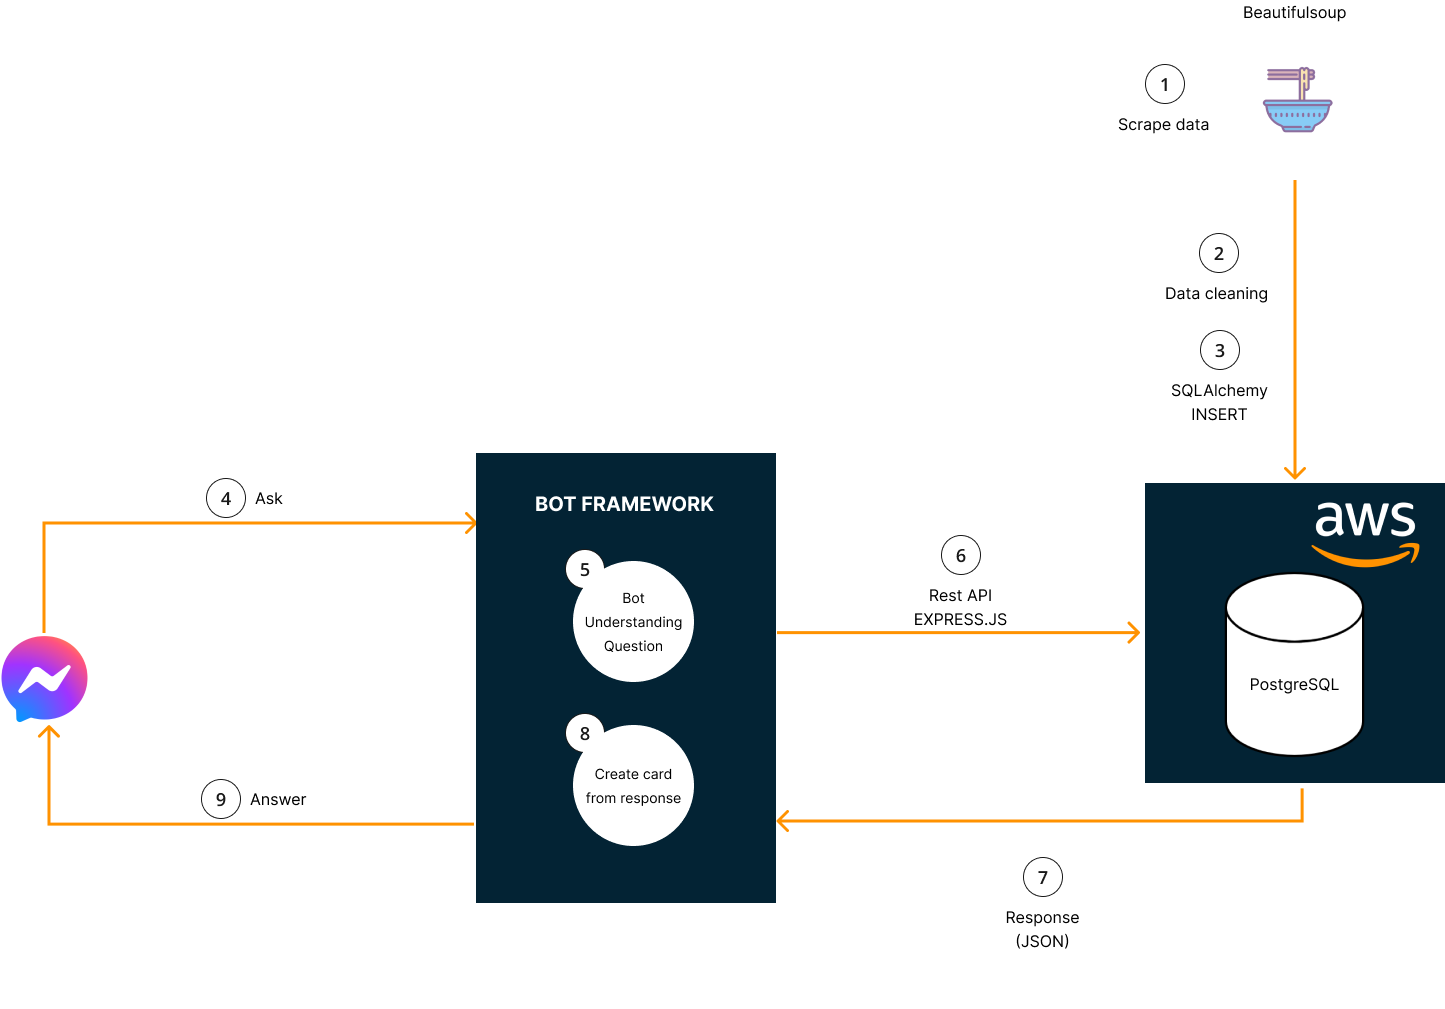
\includegraphics[width = \textwidth-2cm]{images/mainProcess.png}
  \caption{Үндсэн процесс зураглал}\label{mainProcess}
\end{figure}
\\Доорх зурагт чатбот системийн үндсэн процессийн зураглал харагдаж байна. 

\newpage
\subsection{Өгөгдөл цуглуулах}
Үндсэн ашиглагдах өгөгдөл болох ажил олгогчид, ажлын байрны өгөгдлийг \textbf{zangia.mn}-ээс BeautifulSoup ашиглан авсан. Эхлээд вебсайтынхаа HTML бүтцийг нь судалж, авах өгөгдлийнхөө класс утгуудыг (className) олж авах нь зөв юм. Вебсайтаас өгөгдөл цуглуулах 2 үндсэн арга байдгаас өгөгдлийг олж илрүүлж, хаягийг цуглуулах (data crawling) аргаар бүх ангиллуудын хаяг (url)-уудын түүж авна. Харин data scraping нь тэр хооронд олсон бүх хаягуудаараа явж хэрэгтэй агуулгыг цуглуулна. \footnote{Кодын жишээг оруулахад utf-8 формат танихгүй байсан тул монголоос галиглаж бичсэн болно.}
\lstinputlisting[language=Python, firstline=9, lastline=39, caption=Data Link crawling]{code/dataScrapping.py}
Дээрх код нь эхлээд вебсайтруу орж ``filter'' класс доторх ``Салбар, мэргэжил'' гэсэн хэсгээс бүх эцэг категориудыг data crawling хийж авч байна. Үүний дараа хүүхэд категориудыг олж categorySet дотор бүх хаягуудыг хийж хадгалж байна. \footnote{Python хэлний set өгөгдлийн төрөл нь давхацахгүй утгуудын хүснэгт гэж хэлж болно. } Энд categorySet set-ийн элемент нь category төрлийн объект бөгөөд өгөгдлийн сангийн диаграм дээр тодорхойлж өгсөн байгаа. Ингэснээр data crawling-ийг зогсоож, цуглуулсан хаягаасаа өгөгдлөө цуглуулъя.  
\lstinputlisting[language=Python, firstline=41, lastline=52, caption=Өгөгдөл цуглуулах]{code/dataScrapping.py}
Дээрх кодод бүх хүүхэд категориудын дотор агуулагдаж буй зарын мэдээллийг цуглуулж байна. Ингэхдээ эхлээд категори доторх өгөгдлүүд нь хуудаслагдсан (pagination) байх боломжтой бөгөөд хэрэв олон хуудастай байвал хаягуудыг нь угсарч тэдгээрээс ч мөн өгөгдлийг нь цуглуулах ёстой юм. 
Энд dictionary үүсгэхдээ хаягийг нь түлхүүр (key) болгож категори объектыг нь утга(value) болгож хадгалсан. Мэдээж хэрэг dictionary нь түлхүүр давхцахаас сэргийлдэг тул бид ямар нэгэн байдлаар нэг зарын өгөгдлийг 2 удаа цуглуулах эрсдэлгүй болж байна. \footnote{Нэг зарын өгөгдлийг цуглуулахад интернетийн хурдаас хамааран 0.2-оос 0.5 секунтын хугацаа зарцуулдаг}

Харин одоо үүсгэсэн dictionary-оо ашиглан өгөгдлөө SQLAlchemy ашиглан PostgreSQL өгөгдлийн санруугаа хуулна. Ингэхдээ \textbf{upsert} функцийг хүснэгт бүрийн хувьд бичиж тухайн функцийн тусламжтайгаар update эсвэл insert хийх юм. Ангиллын хүснэгтийн хэрхэн upsert хийж байгааг доорх кодын жишээгээр харуулав. 
\lstinputlisting[language=Python, firstline=93, lastline=107, caption=Upsert to PostgreSQL]{code/insert.py}
Дээрх код нь энгийн python програм файлтай харьцаж өөрт цуглуулсан өгөгдлөө хадгалж байна. Нийт өгөгдлийн хүснэгтийг excel файл болгон энд \footnote{\url{https://docs.google.com/spreadsheets/d/1rtATUKhUlleIKaWgFGvqiUWMipsrv-aCWZk-tYmzezU/edit?usp=sharing}} оруулав.
\subsection{Ажлын байрны өгөгдөл}
Zangia.mn ажлын байрны зарын вебсайтаас бакалаврын судалгааны ажлын үечилсэн төлөвлөгөөний дагуу 3 сарын 10-аас эхлэн өгөгдөл цуглуулсан билээ. Цуглуулж, өгөгдлийн сангийн зохиомжийн дагуу дараах утгуудын мэдээллийг CSV файлуудад хадгалж авсан бөгөөд үүнээс цааш бүх өгөгдлийг AWS-EC2 дээр байрших өгөгдлийн санд хадгалж байна.  
Доорх зурагт хамгийн сүүлд буюу 4 сарын 21нд өгөгдлийн цуглуулга хийж 8900 цуглуулж баазруу хийснийг dataGrip-ийн зургаас харж болж байна. 
\begin{figure}[ht]
  \centering
  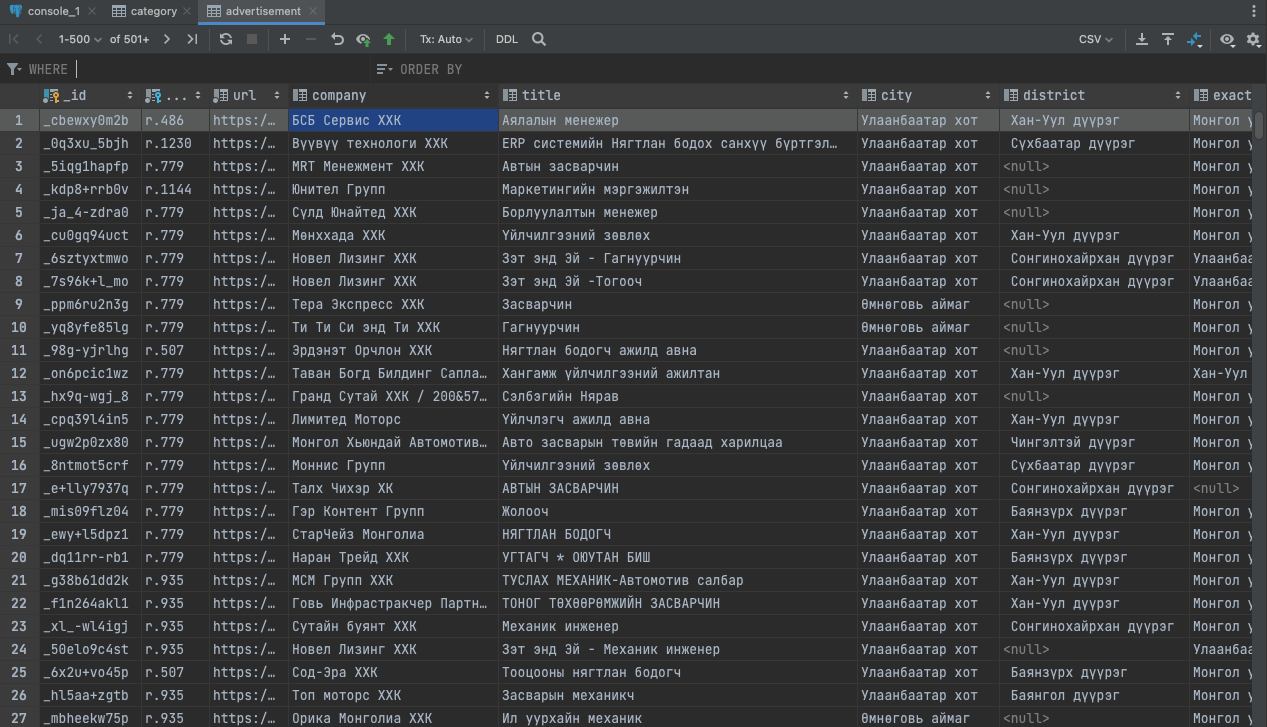
\includegraphics[width=\textwidth-4cm]{images/dataSet.png}
  \caption{Data set}\label{fig:dataSet1}
\end{figure}
Өгөгдөл цуглуулах нь цаг их шаардлагатай, тогтмол ажиллуулж байхад машиныг асаалттай ашиглаж байх шаардлага тулгарах бөгөөд энэхүү асуудлыг виртуал машин болох amazon-ec2-ээ ашиглаж linux машин дээр \textit{crontab} ажиллуулж 7 хоног тутамд тогтмол өгөгдлийг цуглуулж өөр дээрх баазруу цуглуулах юм. Ингэхдээ эх кодоо github-аараа дамжуулан виртуал машин дээрээ ажиллуулж байгаа болно. 
\begin{figure}[ht]
  \centering
  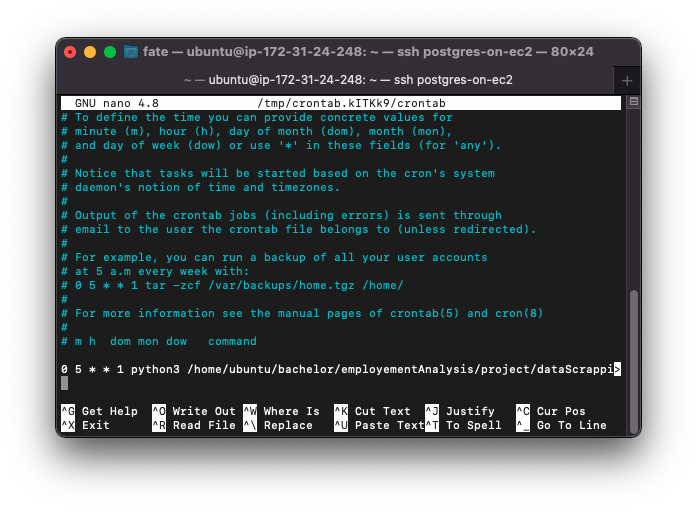
\includegraphics[width=\textwidth-4cm]{images/crontab.png}
  \caption{Виртуал машин дээрх crontab}\label{fig:crontab}
\end{figure}
\newpage
\subsection{Өгөгдлийг нэгтгэх, цэвэрлэх}
Ихэнх цуглуулсан өгөгдөл нь өгөгдлийн сангийн диаграмын дагуу амжилттай цуглуулсан бөгөөд дүн шинжилгээ хийх боломжтой өгөгдлүүдийг тусад нь хадгалж ашигласан болно. Data scrape хийх явцад бүх өгөгдлийг \textit{string} хэлбэрээр цуглуулсан бол өгөгдөлд дүн шинжилгээ хийх явцад энэ нь тохиромжгүй тул цалинг \textit{float} тохиролцох эсэхийг \textit{boolean} болгож өөрчлөв. 
\lstinputlisting[language=Python, firstline=16, lastline=30, caption=Өгөгдөл цэвэрлэх функц]{code/dataVisiulization.py}
\subsection{API ажиллуулах}
Чатбот системд шаардлагатай RestAPI-ийг express.js ашиглан хөгжүүлсэний дараа backend-ийг виртуал машин дээрээ ажиллуулсан. Ингэхдээ node.js -ийн сан болох \textit{pm2}-ийг ашиглав.
\begin{figure}[ht]
  \centering
  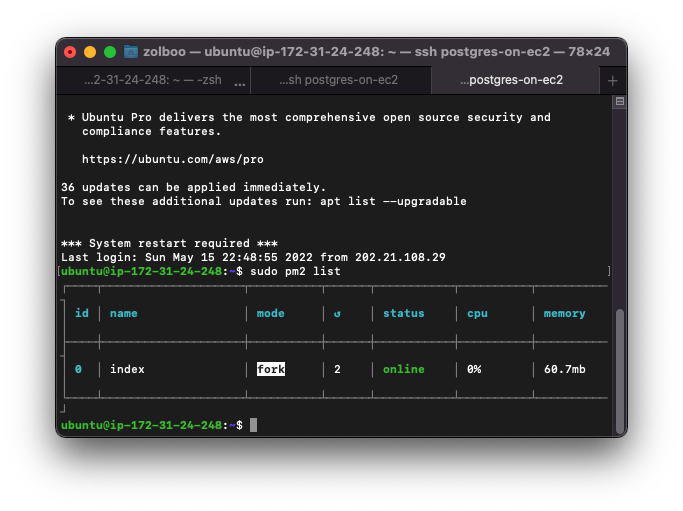
\includegraphics[width=\textwidth-4cm]{images/pm2.png}
  \caption{Виртуал машин дээрх pm2}\label{fig:crontab}
\end{figure}
\newpage
\subsection{Өгөгдлийн статистик}
Өөрчлөлт хийсэн өгөгдөл буюу нийт 8202 зарын өгөгдөл дээрээ дүн шинжилгээ хийж, цаашид үүнийгээ чатбот хөгжүүлэлт, асуулт хариултын загварт тусгахыг зорив.
\\\indent\textbf{Статистик - 1}
\\Энэхүү графикт нийт цалингийн давхардсан утгууд нийт өгөгдлийн хэдэн хувийг эзэлж байгааг харуулж байна. Үүнээс харвал дундаж цалин 1 сая төгрөгөөс 1.5 сая төгрөгийн хооронд байгааг харж болж байна. Энэ нь нийт цалингийн хувийн 50-аас 55-ийг эзэлж байна. 
\begin{figure}[ht]
  \centering
  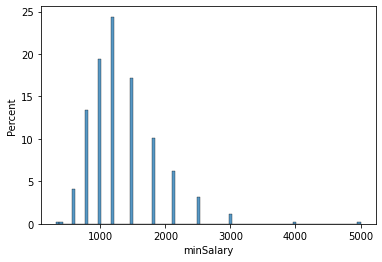
\includegraphics[width=\textwidth]{graphics/2.png}
  \caption{Өгөгдлийн статистик-1}\label{fig:statistics1}
\end{figure}
\\\indent\textbf{Статистик - 2}
\\Доорх графикт нийт цалингийн давхардсан утгуудыг тоолж аль дүүрэгт хамгийн их байгааг өнгөөр нь дүрслэн харуулсан байна. Энэхүү графикаас харвал дундаж цалин буюу 1 сая төгрөгөөс 1.5 сая төгрөгөөр цалинжуулах олон ажлын байр санал болгож байгаа дүүрэг нь Хан-Уул болон Сүхбаатар дүүрэг байна. Ажлын байрны төвлөрөл болон их хотын бүтээгдэхүүн үйлдвэрлэлийн цэгийг Хан-Уул, Сүхбаатар дүүрэг гэж дүгнэж болохоор байна.  
\begin{figure}[ht]
  \centering
  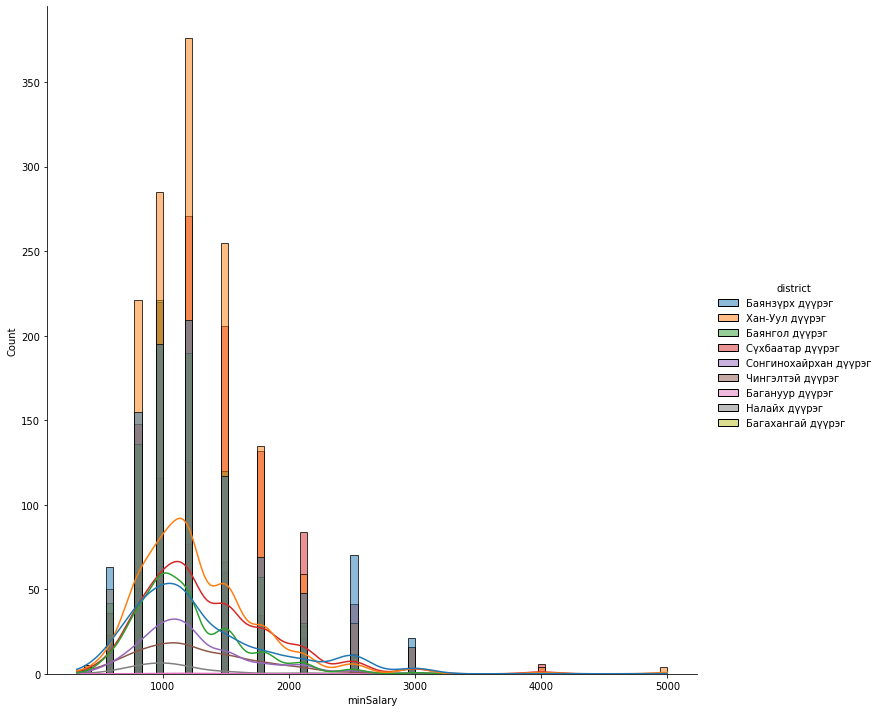
\includegraphics[width=\textwidth]{graphics/3.png}
  \caption{Өгөгдлийн статистик-2}\label{fig:statistics2}
\end{figure}
\newpage
\textbf{Статистик - 3}
\\Өмнөх графикийн дүгнэлтийн адилаар хамгийн их ажлын санал болгож буй дүүрэг нь Хан-Уул, Сүхбаатар дүүрэг байх бөгөөд ажлын байрны шаардах түвшинг хамтад нь харуулсан байна. Үүнээс үзвэл, мэргэжилтэн болон дунд шатны удирдлагын орон тоо эрэлттэй байна гэж үзэж болно. Харин дадлагажигч болон дээд шатны удирдлагын эрэлт харьцангуй бага байгааг харж болж байна.
\begin{figure}[ht]
  \centering
  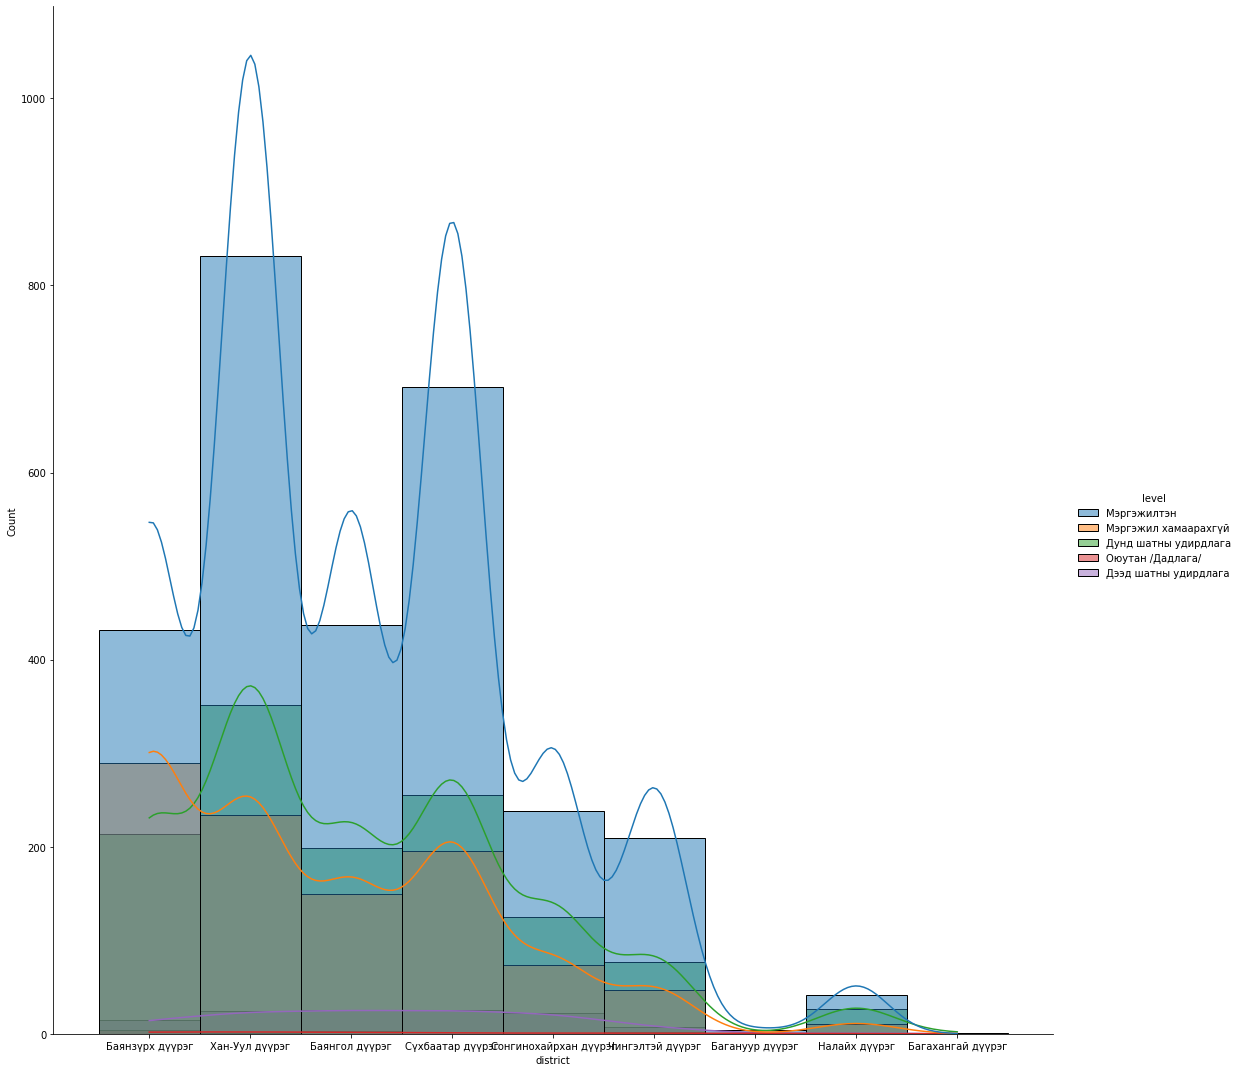
\includegraphics[width=\textwidth]{graphics/4.png}
  \caption{Өгөгдлийн статистик-3}\label{fig:statistics3}
\end{figure}
\newpage
\textbf{Статистик - 4}
\\Энэхүү графикт дүүргүүд харгалзан ямар төрлийн цагийн хуваарьтай ажил санал болгож байгаа болон тэдгээрийн тоотой нь харьцуулан дүрсэлжээ. Эндээс бүтэн цагийн ажилтан болон ээлжийн төрлийн ажлын байр ихэнх хувийг эзэлж байгааг харлаа.
\begin{figure}[ht]
  \centering
  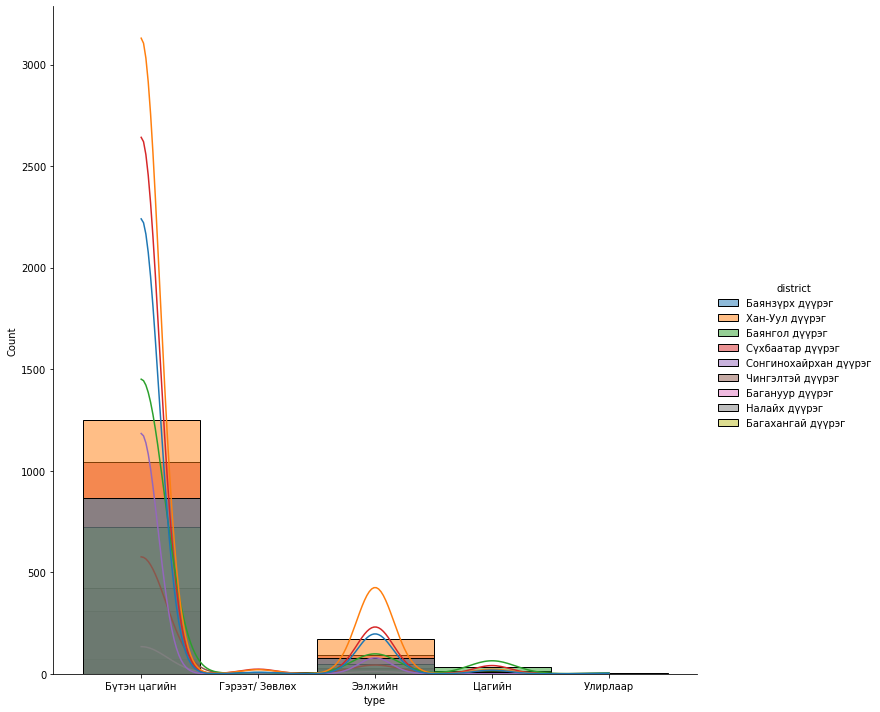
\includegraphics[width=15cm]{graphics/5.png}
  \caption{Өгөгдлийн статистик-4}\label{fig:statistics5}
\end{figure}
\newpage
\textbf{Статистик - 5}
\\Доорх графикаас ажил олгогчид ямар төрлийн цагийн хуваарьтай, хаана ажил санал болгож байгааг 21 аймгаар бүсчлэн өнгөөр илэрхийлсэн байна. Үүнээс дүгнэвэл, Улаанбаатар хотод нягтаршил маш өндөр байгаа бөгөөд ажлын байрны эрэлт аймгуудтай харьцуулахад маш өндөр байна.
\begin{figure}[ht]
  \centering
  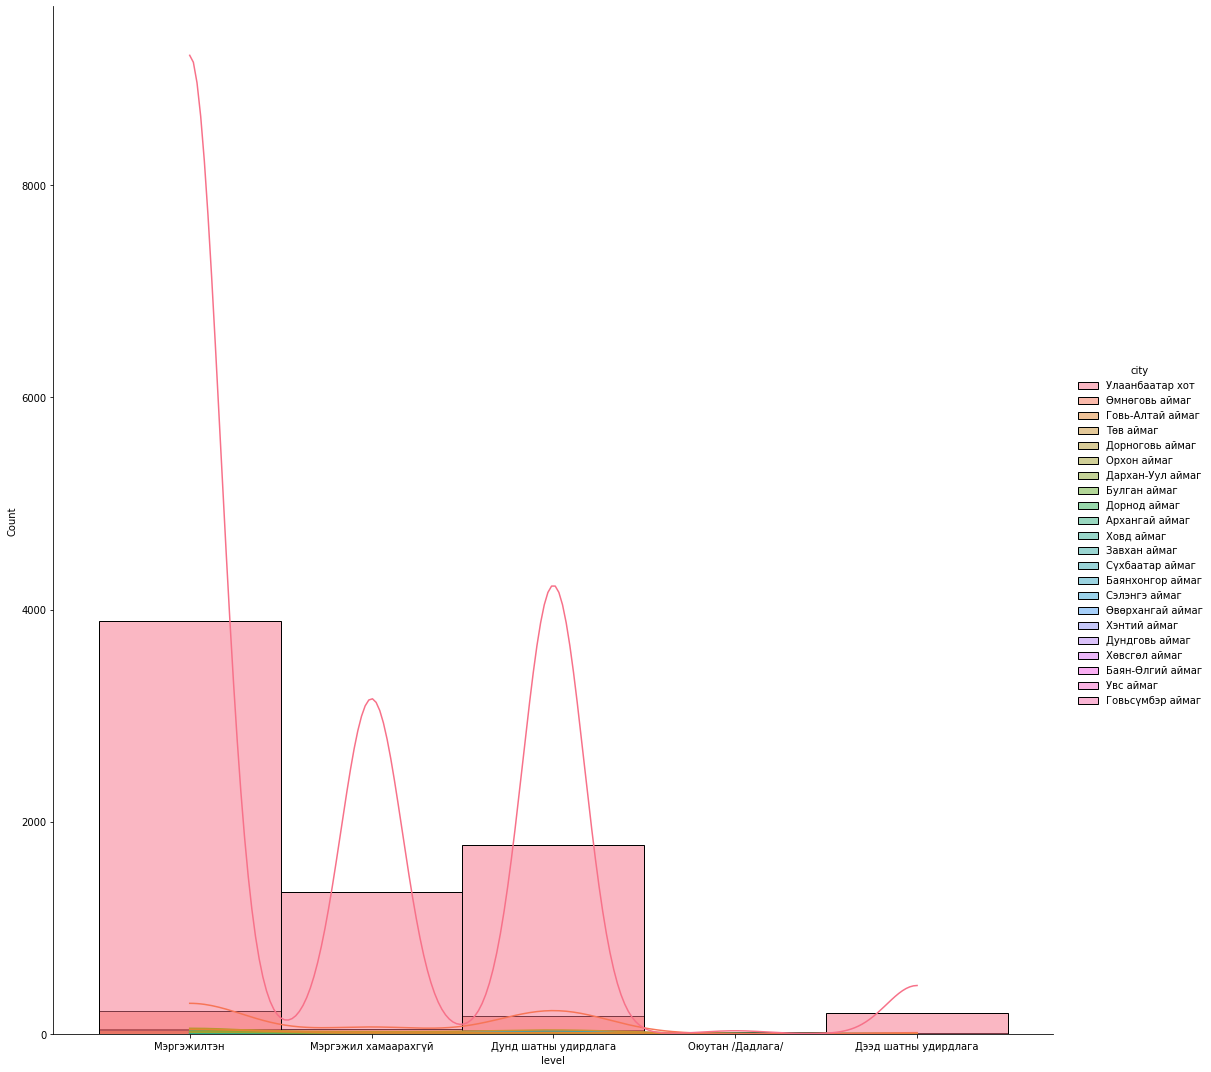
\includegraphics[width=15cm]{graphics/6.png}
  \caption{Өгөгдлийн статистик-5}\label{fig:statistics6}
\end{figure}
\\Дээрх статисткууд дээр үндэслэн, хэрэглэгчдэд хүртээмжтэй, нийтлэг асуултуудыг дараах байдлаар зохиомжлов. 
\begin{figure}[ht]
  \centering
  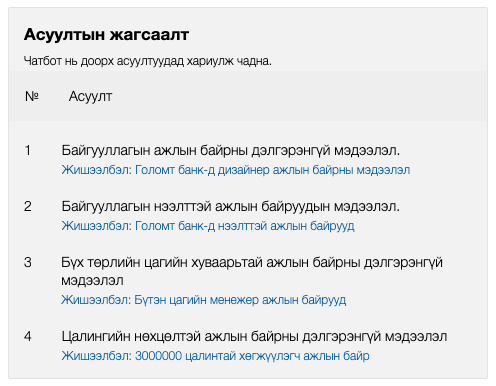
\includegraphics[height=8cm]{images/questions.png}
  \caption{Чатботын хариулж чадах асуултууд}\label{fig:questions}
\end{figure}

\newpage
\subsection{Чатбот хөгжүүлэлт}
Чатбот нь хэрэглэгчийн асуултаас онцлох түлхүүр үгшийг шүүж түүнд тохирох API-ын дагуу AWS дээр байрших өгөгдлийн санруу хүсэлт явуулна. API нь RESTful API бөгөөд express.js ажиллаж үр дүнд JSON өгөгдөл авна. Bot Framework нь тэрхүү өгөгдлийг  \textit{AdaptiveCard}-ын тусламжтайгаар хэрэглэгчдэд ойлгогдохуйц болгон харуулна. Үүний дараа хэрэглэгчид хариултыг буцаах зарчмаар чатбот систем нь ажиллах юм. Энэхүү процессыг алхам алхамаар хэрэгжүүлж тайлбарлая. Хэрэглэгч чатботтой холбогдох үед чатботын хариулж чадах асуултыг харуулна. Хэрэглэгч өөрийн шаардлагад нийцүүлэн асуултаас сонгож чатботоос асууна. 

Эхлээд ашиглагдах REST API-г бэлдэж хэрэглэгчийн асуултад цаг алдалгүй хариулдаг байх шаардлагатай. Иймд express.js ашиглан PostgreSQL-ээс өгөгдлийг JSON-оор авах API бичиж өгсөн. ApiHepler код дээр дурдсанчлан виртуал машин дээр ажиллах бөгөөд нь дараах байдалтай байна. 
\lstinputlisting[language=Python, firstline=5, caption=REST API controller]{code/chatbotCode/rest.js}

Үүний дараа хэрэгэлгчийн асуусан асуултад хариулахад бэлэн болох бөгөөд дараах код нь хэрэглэгчийн асуултыг таньж query үүсгэхэд туслана. Асуултын төрлийг таньсаны дараа асуултаас шаардлагатай query-дэх түлхүүр үгийг олж авна. 
\lstinputlisting[language=Python,  firstline=7, lastline=13, caption=Question-understand классын кодын жишээ 1]{code/chatbotCode/questionUnderstand.js}
\lstinputlisting[language=Python,  firstline=15, lastline=21, caption=Question-understand классын кодын жишээ 2]{code/chatbotCode/questionUnderstand.js}

Ингэж query параметрийг түлхүүр үгийн тусламжтайгаар тодорхойлсны дараа API-аар хандаж өгөгдлийг авахад бэлэн болно. Үүний үр дүнд өгөгдлийн санруу явах query бэлэн болно. 
\lstinputlisting[language=Python,  firstline=33, lastline=37, caption=query бэлтгэх кодын жишнээ]{code/chatbotCode/apiHelper.js}

Дараах кодын хэсэг нь дотоод орчинд ажиллаж буй REST API controller-ыг ашиглан хүсэлт явуулж байна. Үр дүнд нь асуултын хариулт болох JSON объектыг авч байна. 

\lstinputlisting[language=Python,  firstline=10, lastline=30, caption=JSON хүлээж авах кодын жишээ.]{code/chatbotCode/apiHelper.js}
Тухайн үр дүнгээ хэрэглэгчид ойлгогдохоор харуулах шаардлагатай. Үүний тулд Microsoft Bot Framework-ийн картын төрлүүдийг ашигласан. Карт нь олон төрлийн хувилбаруудтай бөгөөд тэр дундаас ”Adaptive Cards”-ыг сонгосон.

\lstinputlisting[language=Python,  firstline=10, lastline=88, caption=Хэрэглэгчийн UI дүрслэх кодын жишээ.]{code/chatbotCode/cardBuilder.js}
Хэрэглэгчид харагдах байдлыг өөрийн хүссэнээр уян хатан зохион байгуулах боломжийг ”Adaptive Cards” олгодог бөгөөд эмх цэгцтэй мэдээллийг хүргэхэд туслах юм. AdaptiveCard нь JSON хэлбэртэй өгөгдлийн хадгалдаг бөгөөд үндсэн 5 төрлийн өгөгдөлтэй байна. Үүнд:
\begin{itemize}
  \item type: Microsoft Botframework нь өөр олон төрлийн картуудтай бөгөөд энд тэдгээрийг зааж өгнө. 
  \item schema: Энд картын эх буюу схемийн хаягийг тодорхойлно.
  \item version: Сонгосон төрлийн картын ямар хувилбарыг ашиглах болохыг зааж өгнө.
  \item body: Энд карт доторх бүх контент буюу мэдээллүүд байна.
  \item actions: Хэрэв карт нь ямар нэг төрлийн товчтой байвал тэдгээр нь юу хийх талаар програмчлана. ( OnClick() г.м )
\end{itemize}

\section{Үр дүн}
Энэхүү хэсэгт асуулт бүрийн хэрэгжүүлэлтийн хэрэглэгчдэд харагдах байдлыг дүрсэлсэн болно. 
\subsection{Угтах текст}
Угтах текстийг шинэ хэрэглэгч болон чатлаагүй удсан хэрэглэгчдэд харуулна. Энэ нь хэрэглэгчийн session дээр суурилсан байна. 
\begin{figure}[ht]
  \centering
  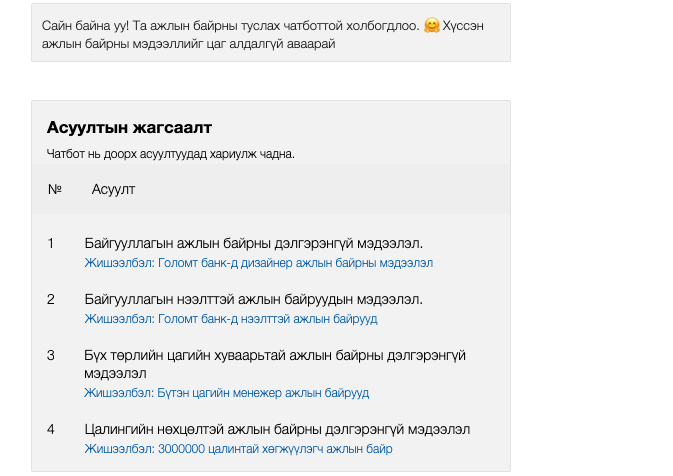
\includegraphics[width=\textwidth]{images/welcomeText.png}
  \caption{Угтах тескт}\label{fig:welcomeUI}
\end{figure}
\subsection{Байгууллагын ажлын байрны дэлгэрэнгүй мэдээлэл}
Ажиллахыг хүссэн байгууллын нэрийг ажлын байрны нэрийн хамтаар асуух нь хамгийн нийтлэг байх бөгөөд тухайн байгууллагын ажлын байрны нэрээр хайлт хийж хэрэглэгчдэд дэлгэрэнгүй мэдээллийг харуулна. 
\begin{itemize}
  \item Голомт Банк-д дизайнер ажлын байрны дэлгэрэнгүй мэдээлэл асуултын хариулт хэрэглэгчид харагдах байдал:
\end{itemize}
\begin{figure}[ht]
  \centering
  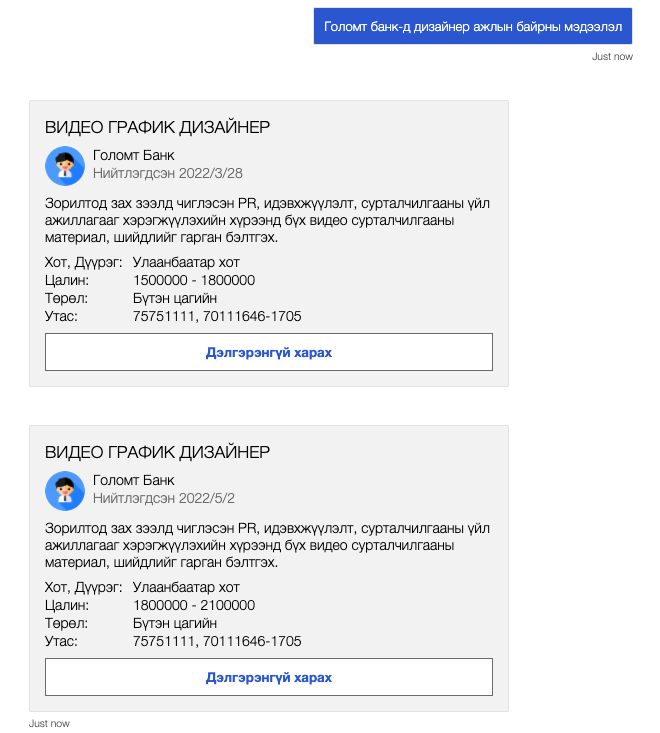
\includegraphics[width=\textwidth-4cm]{images/question1.png}
  \caption{<Байгууллага>-д <ажил> ажлын байрны мэдээлэл?}\label{fig:quest1}
\end{figure}
Хэрэв тухайн байгууллагад хайсан ажлын байрны нээлттэй зарын мэдээлэл байхгүй тохиолдолд байгууллагын нээлттэй ажлын байруудын мэдээллийг дүрслэнэ.
\begin{figure}[ht]
  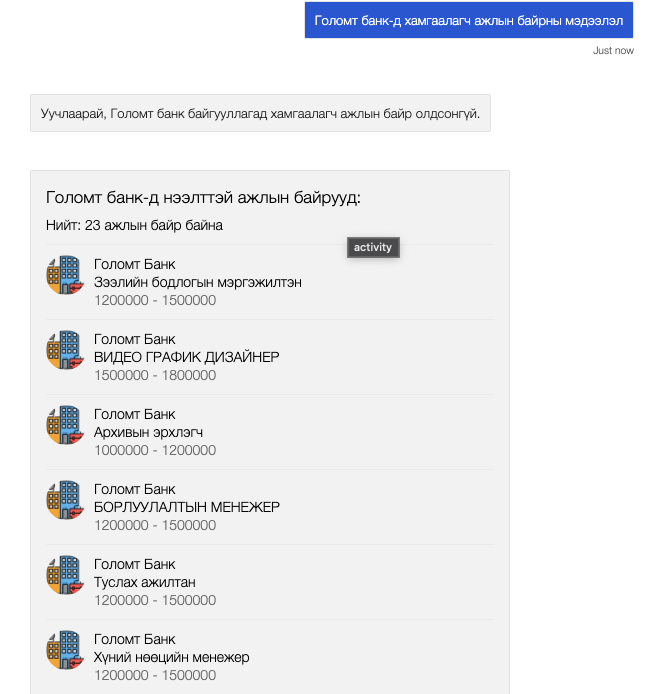
\includegraphics[width=\textwidth-4cm]{images/question1-2.png}
  \caption{Бусад ажлын байрууд} \label{fig:quest1-2}
\end{figure}
\newpage
\subsection{Байгууллагын нээлттэй ажлын байруудын мэдээлэл}
Ажиллахыг хүссэн байгууллын нэрийн дагуу нээлттэй ажлын байруудыг харах боломжтой.
\begin{itemize}
  \item Голомт Банк-д нээлттэй ажлын байруудын мэдээлэл асуултын хариулт хэрэглэгчдэд харагдах байдал:
\end{itemize}
\begin{figure}[ht]
  \centering
  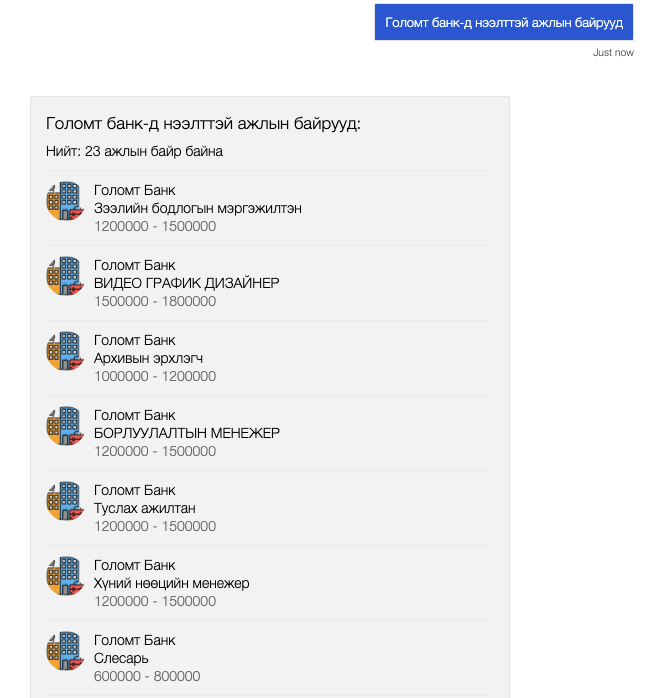
\includegraphics[width=\textwidth-4cm]{images/question2.png}
  \caption{<Байгууллага>-д нээлттэй ажлын байрууд?}\label{fig:quest2}
\end{figure}
\newpage
\subsection{Бүх төрлийн цагийн хуваарьтай ажлын байрны дэлгэрэнгүй мэдээлэл}
Ажиллахыг хүссэн ажлын байрны дагуу ажиллах цагийн хувиариар шүүж харах боломжтой байна. Бүх боломжит ажлын байруудын дэлгэрэнгүй мэдээллийг харуулна.
\begin{itemize}
  \item Бүтэн цагийн тогооч ажлын байр асуултын хариулт хэрэглэгчдэд харагдах байдал:
\end{itemize}
\begin{figure}[ht]
  \centering
  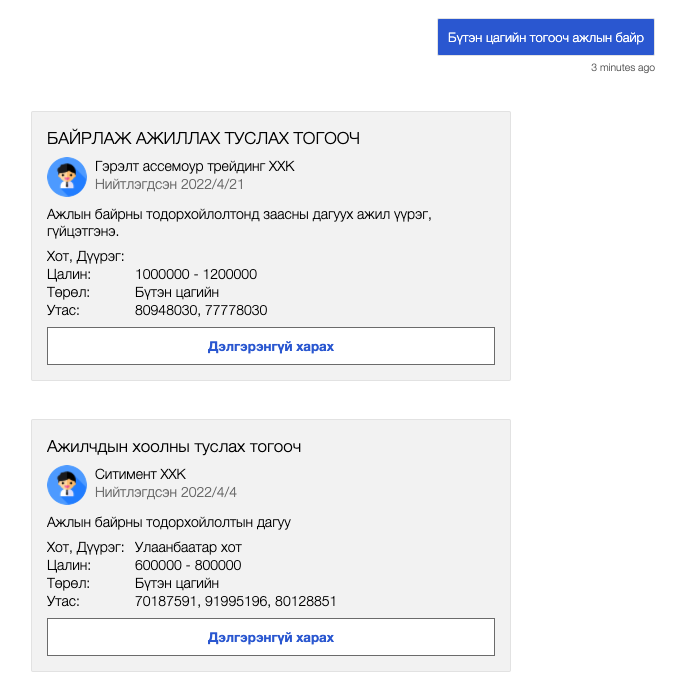
\includegraphics[width=\textwidth-3.5cm]{images/question3.png}
  \caption{<Ажиллах цаг> цагийн <ажил> ажлын байр?}\label{fig:quest3}
\end{figure}
\newpage
\subsection{Цалингийн нөхцөлтэй ажлын байрны дэлгэрэнгүй мэдээлэл}
Ажиллахыг хүссэн ажлын байрны дагуу цалингийн хэмжээгээр шүүж харах боломжтой байна. Бүх боломжит ажлын байрыг жагсаалт хэлбэрээр харуулна.
\begin{itemize}
  \item Бүтэн цагийн тогооч ажлын байр асуултын хариулт хэрэглэгчдэд харагдах байдал:
\end{itemize}
\begin{figure}[ht]
  \centering
  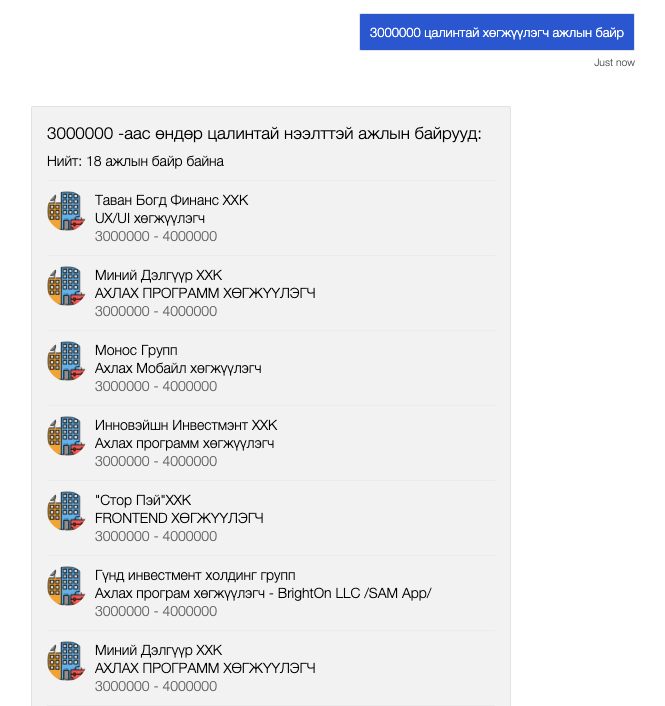
\includegraphics[width=\textwidth-4cm]{images/question4.png}
  \caption{<Цалин> цалинтай <ажил> ажлын байр?}\label{fig:quest4}
\end{figure}